\chapter{Implementación y despliegue}
El servidor utilizado para el ambiente de producción es una máquina virtual proveída por Ormuco, consiste en un equipo de 4 núcleos con 16GB de memoria RAM y Ubuntu Server 16.04 como Sistema Operativo. 

\section{Implementación Actual}
Desde su despliegue inicial, ALTEM ha tenido una implementación de servidor web tradicional. Se utiliza \textbf{Nginx} como servidor web, el cual se encarga de proveer el cliente web a los usuarios que se conecten al servidor desde su navegador web.
El servidor web posee una configuración que cumple con los estándares básicos de funcionamiento y seguridad de una página web:

\begin{itemize}
    \item Enrutamiento por medio de su propio dominio (\url{altem.utb.edu.co})
    \item Certificado SSL Válido
\end{itemize}

Dentro del sistema operativo, se encuentran instaladas todas las dependencias necesarias para correr ALTEM, tales como Node.JS, PHP y MySQL. Todas estas dependencias comparten el mismo sistema operativo y ambiente de producción. 

Todas las conexiones internas entre componentes se referencian bajo localhost debido a que todo se encuentra dentro de la misma máquina.

Esta implementación hace que el despliegue sea difícil de mantener ya que no existe la posibilidad de pre-escribir las configuraciones de cada uno de los servicios, lo que hace el proceso de despliegue mucho más lento, pero crea un mejor rendimiento debido a que no existe una capa de virtualización como se ve en arquitecturas de despliegue más modernas.

\section{Implementación Propuesta}
Se propuso cambiar la implementación del despliegue por una más moderna, añadiendo una capa de DevOps.
ALTEM, al ser de una arquitectura modular, permite automatizar el proceso de implementación y despliegue de la aplicación en el servidor, por medio del aislamiento de cada uno de estos módulos utilizando contenedores.

Se planteó una Arquitectura compuesta por 3 contenedores los cuales corren en Docker, estos estarían funcionando en la misma máquina, pero en ambientes completamente aislados como se espera al usar contenedores. Estos contenedores se comunicarían a través de una red privada virtual proveída por el mismo Docker.

La principal ventaja de utilizar contenedores es que se puede hacer un despliegue con una sola instrucción, ya que, para cada contenedor se pueden pre-escribir sus configuraciones de inicio las cuales son ejecutadas al momento de que se instancia el contenedor. 

\subsection{Contenedor de Bases de Datos}
Este contendedor utiliza una imagen de Docker optimizada para MySQL, esto nos permite correr la base de datos en su propio entorno aislado, sin tener ninguna clase de interferencia con ninguna variable de entorno o configuración externa.
Esta imagen cuenta con 2 volúmenes, en los que se almacena la información y la configuración respectivamente. También cuenta con un puerto abierto el cual permite la comunicación con los otros servicios.

\begin{figure}[H]
    \centering
    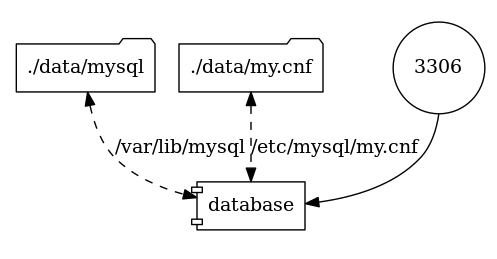
\includegraphics[width=0.7\textwidth]{img/db_container.png}
    \caption{Contenedor de Base de Datos en Docker }
\end{figure}

\subsection{Contenedor de la API en PHP}
Este contenedor utiliza una imagen de Docker optimizada para correr PHP y Laravel, y dos volúmenes, uno compartido y otro aislado, el compartido es en donde se encuentra todo el código fuente y el aislado es en donde está la configuración del entorno.

\begin{figure}[H]
    \centering
    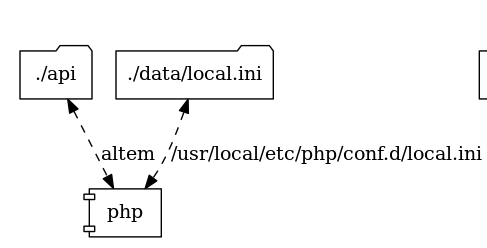
\includegraphics[width=0.7\textwidth]{img/api_container.png}
    \caption{Contenedor de la API en Docker}
\end{figure}

\subsection{Contenedor del Servidor Web}
Este contenedor utiliza una imagen optimizada para correr el servidor web Nginx y posee dos volúmenes, uno compartido y otro aislado, el volumen compartido es el mismo que se comparte en el contenedor de la API, Nginx necesita acceso al código fuente para poder manejar las solicitudes que vienen del cliente. Este contenedor posee 2 puertos abiertos, uno para el acceso al cliente (puerto 80) y el otro para el acceso del cliente a la API. (Puerto 8000).

\begin{figure}[H]
    \centering
    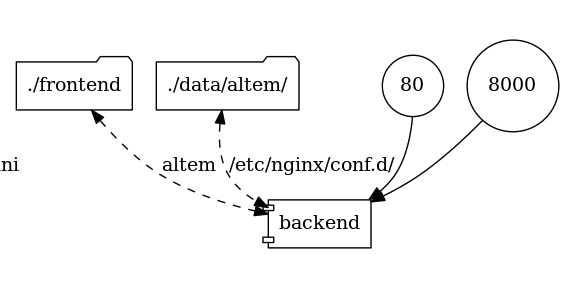
\includegraphics[width=0.7\textwidth]{img/ws_container.png}
    \caption{Contenedor del Servidor Web en Docker}
\end{figure}

\subsection{Fallas en la Implementación}
Esta implementación requirió de un cambio en la estructura de carpetas que se venía manejando en el proyecto, con el fin de aislar completamente el código fuente del servidor del código fuente del cliente. 
Esta implementación quedó propuesta en el repositorio de la universidad bajo la rama \textbf{devopsensable}, pero nunca se llegó a implementar debido a la existencia de unas fallas en la configuración del contenedor de la API. Se cree que el problema está siendo ocasionado debido a que la versión especificada de Laravel en la configuración no es la adecuada.